
% This LaTeX was auto-generated from MATLAB code.
% To make changes, update the MATLAB code and republish this document.

\documentclass{article}
\usepackage{graphicx}
\usepackage{color}

\sloppy
\definecolor{lightgray}{gray}{0.5}
\setlength{\parindent}{0pt}

\begin{document}

    
    \begin{verbatim}
clear all
import brml.*
% Do Metropolis sampling:
L=200000; % number of samples
x(:,1)=rand(2,1); % intial sample
s=2; % width of Metropolis candidate distribution
for l=2:L
	x(:,l)=metropolis(x(:,l-1),s,'fgprob');
end

figure
dat = hist3(x');
dat = dat+1;
dat = dat/sum(sum(dat));
dat = rot90(dat,1);
heatmap(0:.1:.9,.9:-.1:0,dat)

F = mean(x(1,:));
G = mean(x(2,:));
expected = F*G
\end{verbatim}

        \color{lightgray} \begin{verbatim}
ans = 

  HeatmapChart with properties:

        XData: {10�1 cell}
        YData: {10�1 cell}
    ColorData: [10�10 double]

  Use GET to show all properties


expected =

    0.4703

\end{verbatim} \color{black}
    
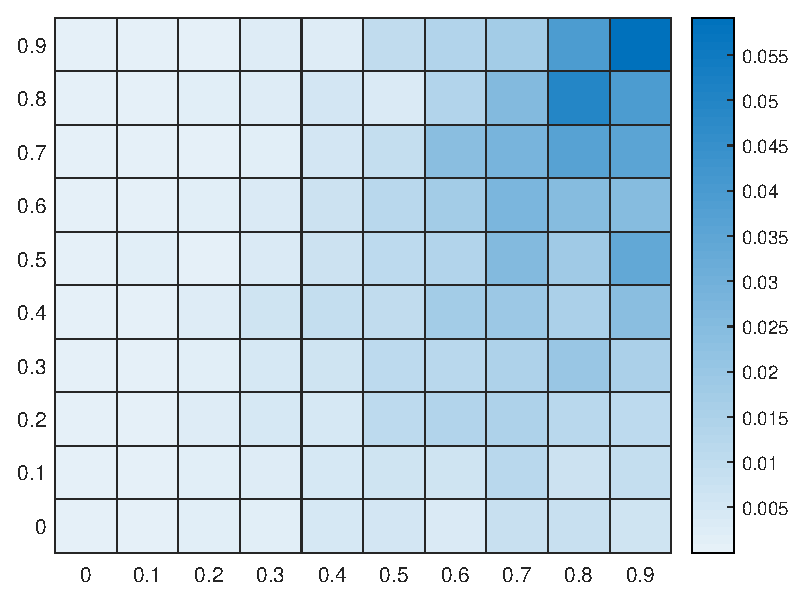
\includegraphics [width=4in]{hw5p3_01.eps}



\end{document}
    
